\documentclass[aspectratio=169, 11pt]{beamer}

% ========== 主题设置 ==========
\usetheme{Madrid}
\usecolortheme{whale}
\setbeamertemplate{navigation symbols}{}
\setbeamertemplate{footline}[frame number]

% ========== 包 ==========
\usepackage{tikz}
\usetikzlibrary{arrows.meta, positioning, shapes.geometric, calc, fit, backgrounds}
\usepackage{booktabs}
\usepackage{graphicx}
\usepackage{amsmath}
\usepackage{xcolor}
\usepackage{subcaption}

% ========== 颜色定义 ==========
\definecolor{highlight}{RGB}{255, 100, 100}      % 当前工作模块（红色高亮）
\definecolor{completed}{RGB}{100, 200, 100}      % 已完成模块（绿色）
\definecolor{pending}{RGB}{200, 200, 200}        % 待完成模块（灰色）
\definecolor{inprogress}{RGB}{100, 150, 255}     % 进行中（蓝色）

% ========== 标题信息 ==========
\title{Weekly Progress Report}
\subtitle{Week 9: Physical Robot Arm Testing \& EEG-Based Control Integration}
\author{Student ID: 11314389}
\institute{BCI Control System Project}
\date{March 4, 2026}

\begin{document}

% ========== 标题页 ==========
\begin{frame}
    \titlepage
\end{frame}

% ========== Slide 1: 系统架构图 ==========
\begin{frame}{System Overview: Current Focus}
    \begin{center}
    \resizebox{0.95\textwidth}{!}{%
    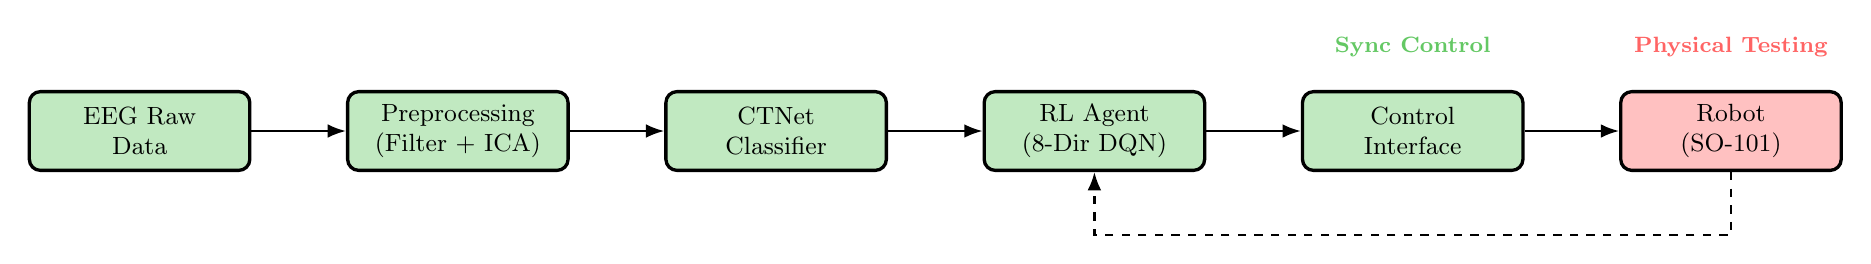
\begin{tikzpicture}[
        node distance=8mm and 12mm,
        block/.style={rectangle, rounded corners, draw, very thick,
                      minimum width=28mm, minimum height=10mm,
                      align=center, font=\small},
        arrow/.style={-Latex, thick},
    ]
        \node[block, fill=completed!40] (raw) {EEG Raw\\Data};
        \node[block, fill=completed!40, right=of raw] (prep) {Preprocessing\\(Filter + ICA)};
        \node[block, fill=completed!40, right=of prep] (ctnet) {CTNet\\Classifier};
        \node[block, fill=completed!40, right=of ctnet] (dqn) {RL Agent\\(8-Dir DQN)};
        \node[block, fill=completed!40, right=of dqn] (ctrl) {Control\\Interface};
        \node[block, fill=highlight!40, right=of ctrl] (robot) {Robot\\(SO-101)};
        
        \draw[arrow] (raw) -- (prep);
        \draw[arrow] (prep) -- (ctnet);
        \draw[arrow] (ctnet) -- (dqn);
        \draw[arrow] (dqn) -- (ctrl);
        \draw[arrow] (ctrl) -- (robot);
        
        \draw[arrow, dashed] (robot.south) -- ++(0,-8mm) -| (dqn.south);
        
        \node[above=3mm of robot, highlight, font=\footnotesize\bfseries] {Physical Testing};
        \node[above=3mm of ctrl, completed, font=\footnotesize\bfseries] {Sync Control};
        
    \end{tikzpicture}}
    \end{center}
    
    \vspace{3mm}
    \begin{columns}[T]
        \column{0.5\textwidth}
        \textbf{Legend:}
        \begin{itemize}
            \item[\textcolor{completed}{\rule{8pt}{8pt}}] Completed
            \item[\textcolor{inprogress}{\rule{8pt}{8pt}}] In Progress
        \end{itemize}
        \column{0.5\textwidth}
        \begin{itemize}
            \item[\textcolor{highlight}{\rule{8pt}{8pt}}] \textbf{This Week's Focus}
            \item[\textcolor{pending}{\rule{8pt}{8pt}}] Pending
        \end{itemize}
    \end{columns}
\end{frame}

% ========== Slide 2: 本周目标 ==========
\begin{frame}{This Week's Objectives}
    \begin{block}{Goals}
        \begin{enumerate}
            \item Test 8-direction movement patterns on physical SO-101 robot arm
            \item Implement synchronized joint movement for smooth homing/return
            \item Integrate EEG subject sequences with physical robot control
            \item Compare simulated vs physical robot trajectories
        \end{enumerate}
    \end{block}
    
    \vspace{5mm}
    
    \begin{alertblock}{Key Question to Address}
        Can the physical robot arm accurately reproduce the movement patterns designed in simulation, and how does EEG-based control perform on real hardware?
    \end{alertblock}
\end{frame}

% ========== Slide 3: 方法/实现 ==========
\begin{frame}{Methods \& Implementation}
    \begin{columns}[T]
        \column{0.5\textwidth}
        \textbf{Synchronized Joint Control:}
        \begin{itemize}
            \item All joints arrive at target simultaneously
            \item Velocity calculated based on distance
            \item Velocity boost for loaded joints (1.3x-1.5x)
        \end{itemize}
        
        \vspace{3mm}
        \textbf{Velocity Synchronization:}
        \begin{equation*}
            v_j = \frac{d_j}{t_{total}} \times \text{boost}_j
        \end{equation*}
        
        \column{0.5\textwidth}
        \textbf{Implementation Files:}
        \begin{itemize}
            \item \texttt{test\_8dir\_comprehensive.py}
            \item \texttt{eeg\_physical\_control.py}
            \item \texttt{serial\_go\_home\_sync.py}
            \item \texttt{serial\_go\_return\_sync.py}
        \end{itemize}
        
        \vspace{3mm}
        \textbf{Test Patterns (6 types):}
        \begin{itemize}
            \item Horizontal, Vertical
            \item Diagonal (2 patterns)
            \item Square CW/CCW
        \end{itemize}
    \end{columns}
\end{frame}

% ========== Slide 4: 8Dir Comprehensive Test - Horizontal/Vertical ==========
\begin{frame}{Physical Robot Test: Horizontal \& Vertical Movement}
    \begin{columns}[T]
        \column{0.5\textwidth}
        \textbf{Horizontal Movement:}
        \begin{center}
            
\includegraphics[width=0.95\textwidth]{../outputs/8dir_comprehensive_test/a_horizontal.png}
        \end{center}
        
        \column{0.5\textwidth}
        \textbf{Vertical Movement:}
        \begin{center}
            
\includegraphics[width=0.95\textwidth]{../outputs/8dir_comprehensive_test/b_vertical.png}
        \end{center}
    \end{columns}
    
    \vspace{2mm}
    \textbf{Observations:}
    \begin{itemize}
        \item Smooth trajectory with consistent velocity
        \item Y/Z positions tracked accurately to targets
    \end{itemize}
\end{frame}

% ========== Slide 5: 8Dir Comprehensive Test - Diagonal ==========
\begin{frame}{Physical Robot Test: Diagonal Movement}
    \begin{columns}[T]
        \column{0.5\textwidth}
        \textbf{Diagonal UL-DR:}
        \begin{center}
            
\includegraphics[width=0.95\textwidth]{../outputs/8dir_comprehensive_test/c_diagonal_ul_dr.png}
        \end{center}
        
        \column{0.5\textwidth}
        \textbf{Diagonal UR-DL:}
        \begin{center}
            
\includegraphics[width=0.95\textwidth]{../outputs/8dir_comprehensive_test/d_diagonal_ur_dl.png}
        \end{center}
    \end{columns}
    
    \vspace{2mm}
    \textbf{Observations:}
    \begin{itemize}
        \item Both Y and Z change simultaneously (true diagonal motion)
        \item 8-direction action space enables efficient diagonal paths
    \end{itemize}
\end{frame}

% ========== Slide 6: 8Dir Comprehensive Test - Square ==========
\begin{frame}{Physical Robot Test: Square Movement Patterns}
    \begin{columns}[T]
        \column{0.5\textwidth}
        \textbf{Square Clockwise:}
        \begin{center}
            
\includegraphics[width=0.95\textwidth]{../outputs/8dir_comprehensive_test/e_square_cw.png}
        \end{center}
        
        \column{0.5\textwidth}
        \textbf{Square Counter-Clockwise:}
        \begin{center}
            
\includegraphics[width=0.95\textwidth]{../outputs/8dir_comprehensive_test/f_square_ccw.png}
        \end{center}
    \end{columns}
    
    \vspace{2mm}
    \textbf{Observations:}
    \begin{itemize}
        \item Complex multi-target sequences completed successfully
        \item All 4 corners reached with good precision
    \end{itemize}
\end{frame}

% ========== Slide 7: 8Dir All Patterns Overview ==========
\begin{frame}{Physical Robot Test: All Patterns Overview}
    \begin{center}
        
\includegraphics[width=0.85\textwidth]{../outputs/8dir_comprehensive_test/all_pos_vs_time.png}
    \end{center}
    
    \textbf{Summary:} All 6 movement patterns executed successfully on physical robot
\end{frame}

% ========== Slide 8: EEG Physical Control - Subjects 1-3 ==========
\begin{frame}{EEG-Based Physical Control: Subjects 1-3}
    \begin{columns}[T]
        \column{0.33\textwidth}
        \textbf{Subject 1 (Horizontal):}
        \begin{center}
            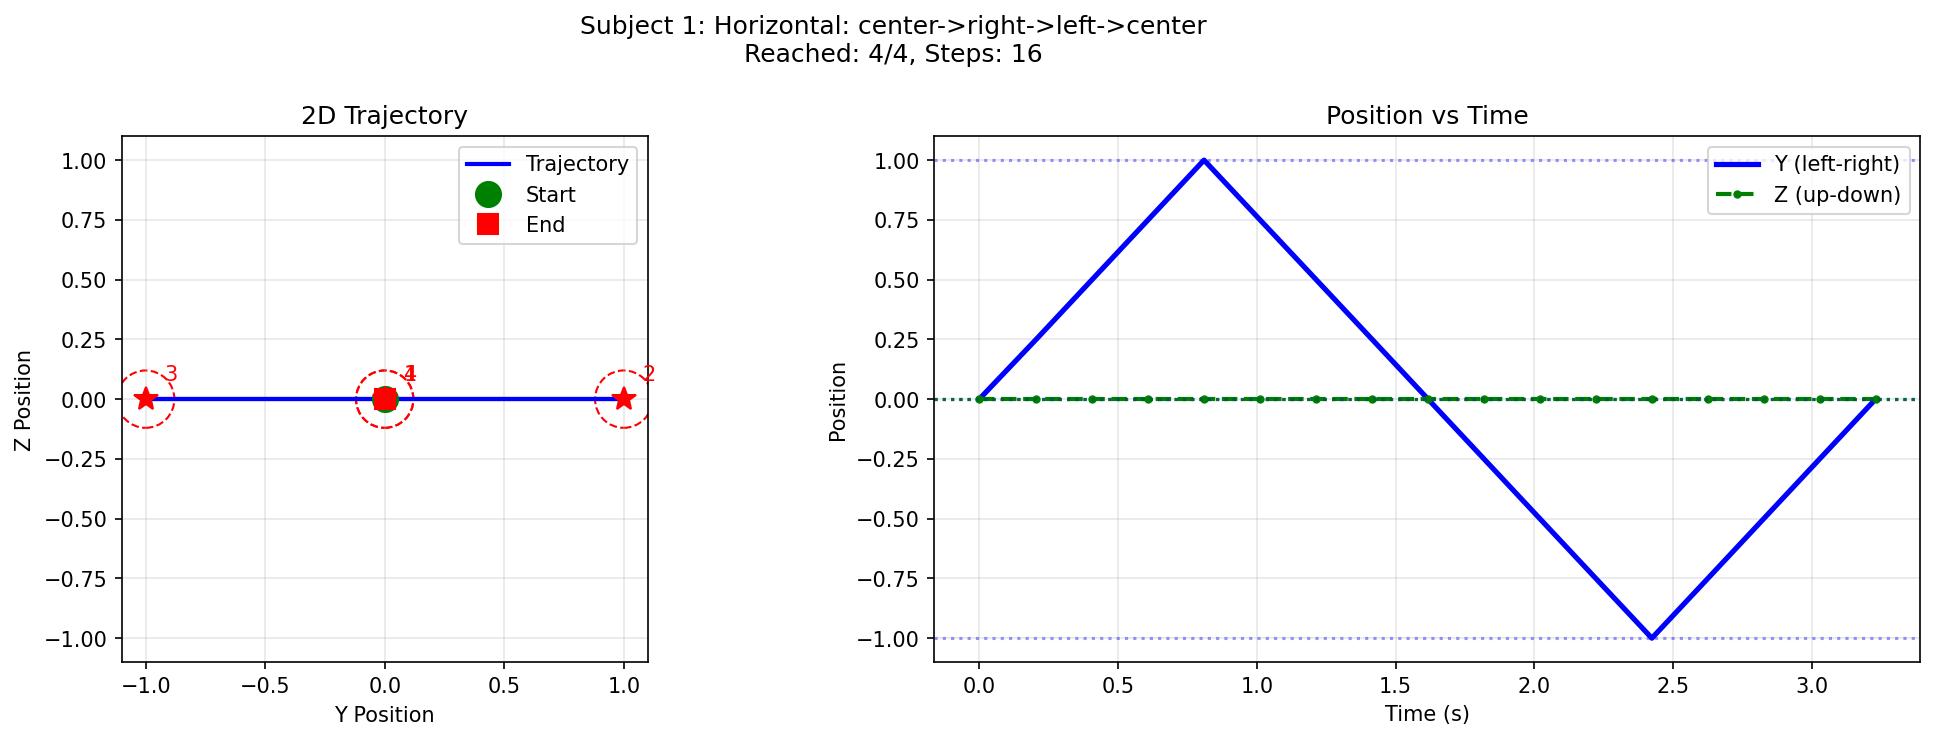
\includegraphics[width=\textwidth]{../outputs/eeg_physical_control/subject_1.png}
        \end{center}
        
        \column{0.33\textwidth}
        \textbf{Subject 2 (Vertical):}
        \begin{center}
            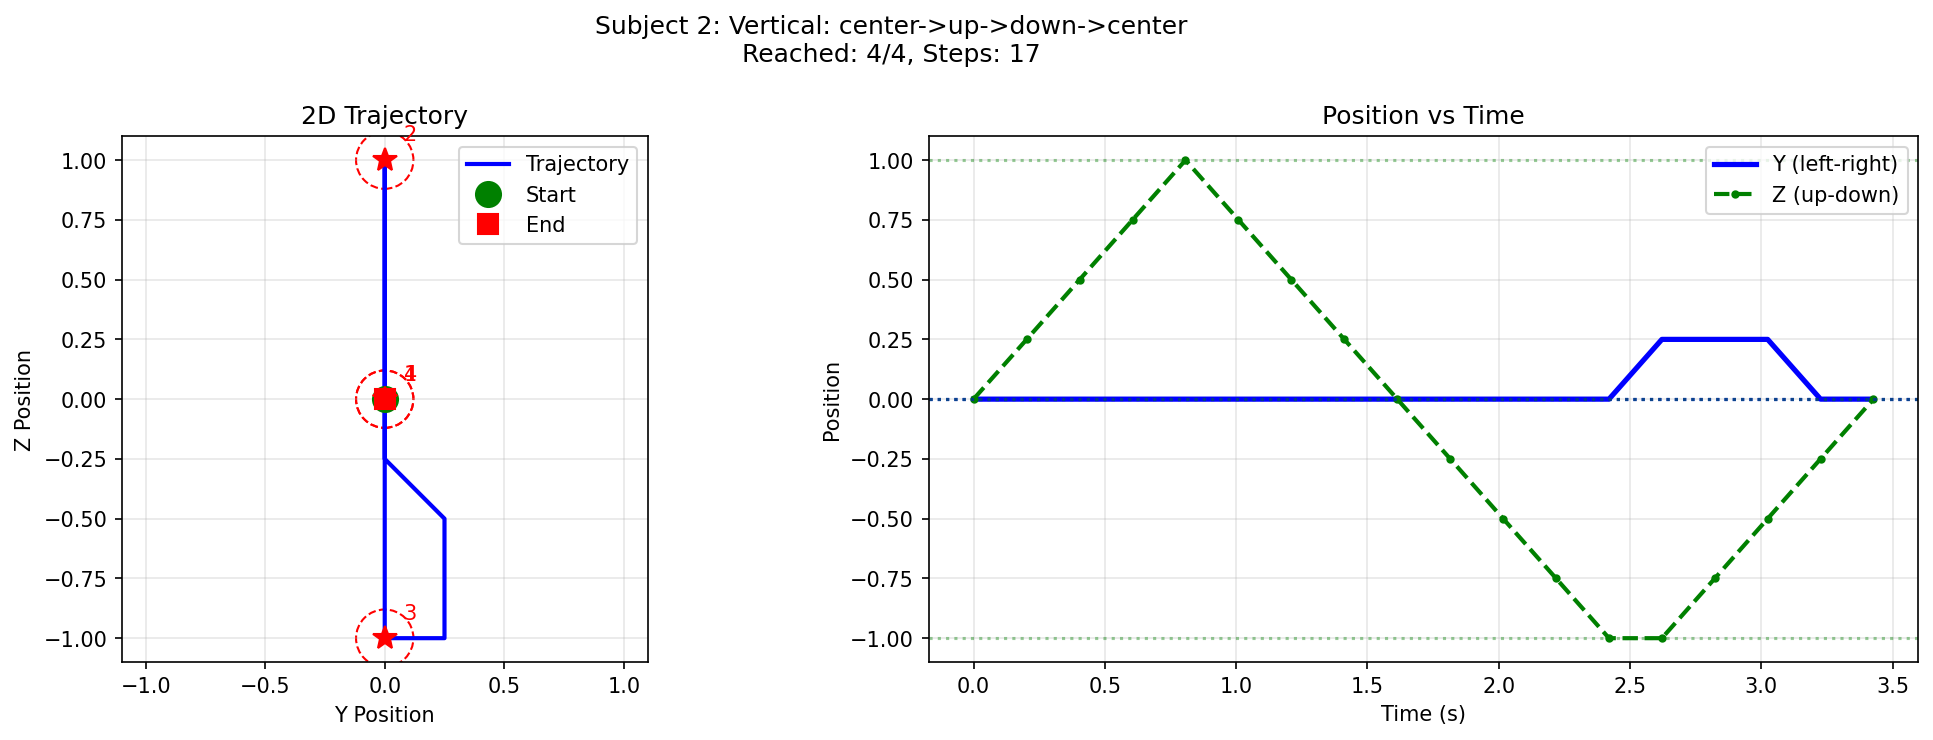
\includegraphics[width=\textwidth]{../outputs/eeg_physical_control/subject_2.png}
        \end{center}
        
        \column{0.33\textwidth}
        \textbf{Subject 3 (Diagonal):}
        \begin{center}
            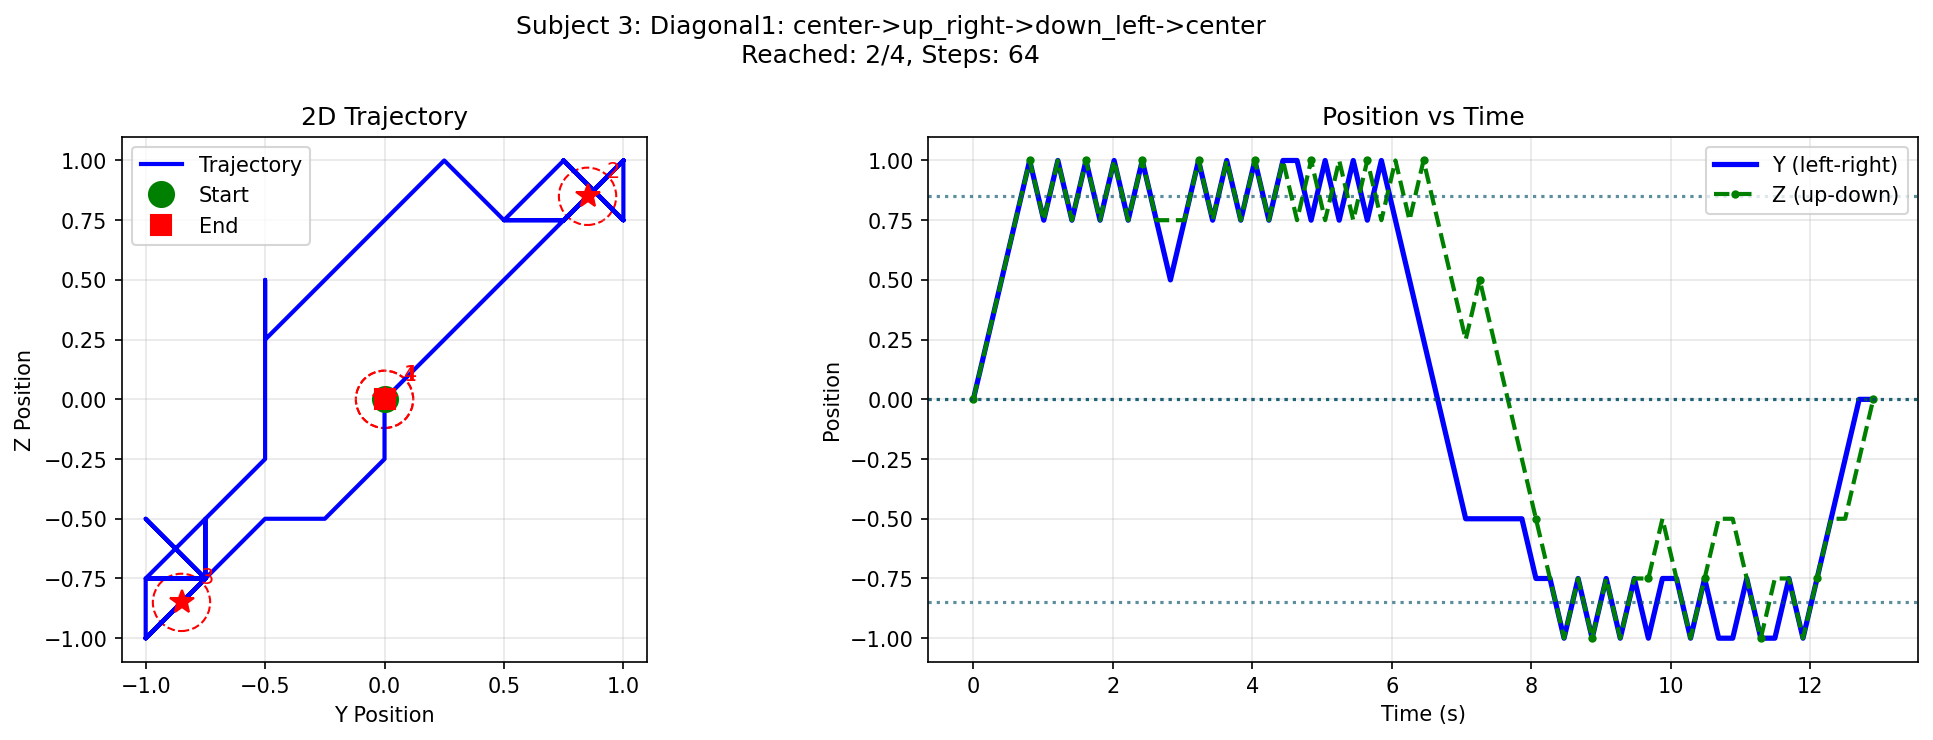
\includegraphics[width=\textwidth]{../outputs/eeg_physical_control/subject_3.png}
        \end{center}
    \end{columns}
    
    \vspace{2mm}
    \textbf{Note:} EEG classification includes 10\% noise to simulate real-world conditions
\end{frame}

% ========== Slide 9: EEG Physical Control - Subjects 4-6 ==========
\begin{frame}{EEG-Based Physical Control: Subjects 4-6}
    \begin{columns}[T]
        \column{0.33\textwidth}
        \textbf{Subject 4 (Diagonal 2):}
        \begin{center}
            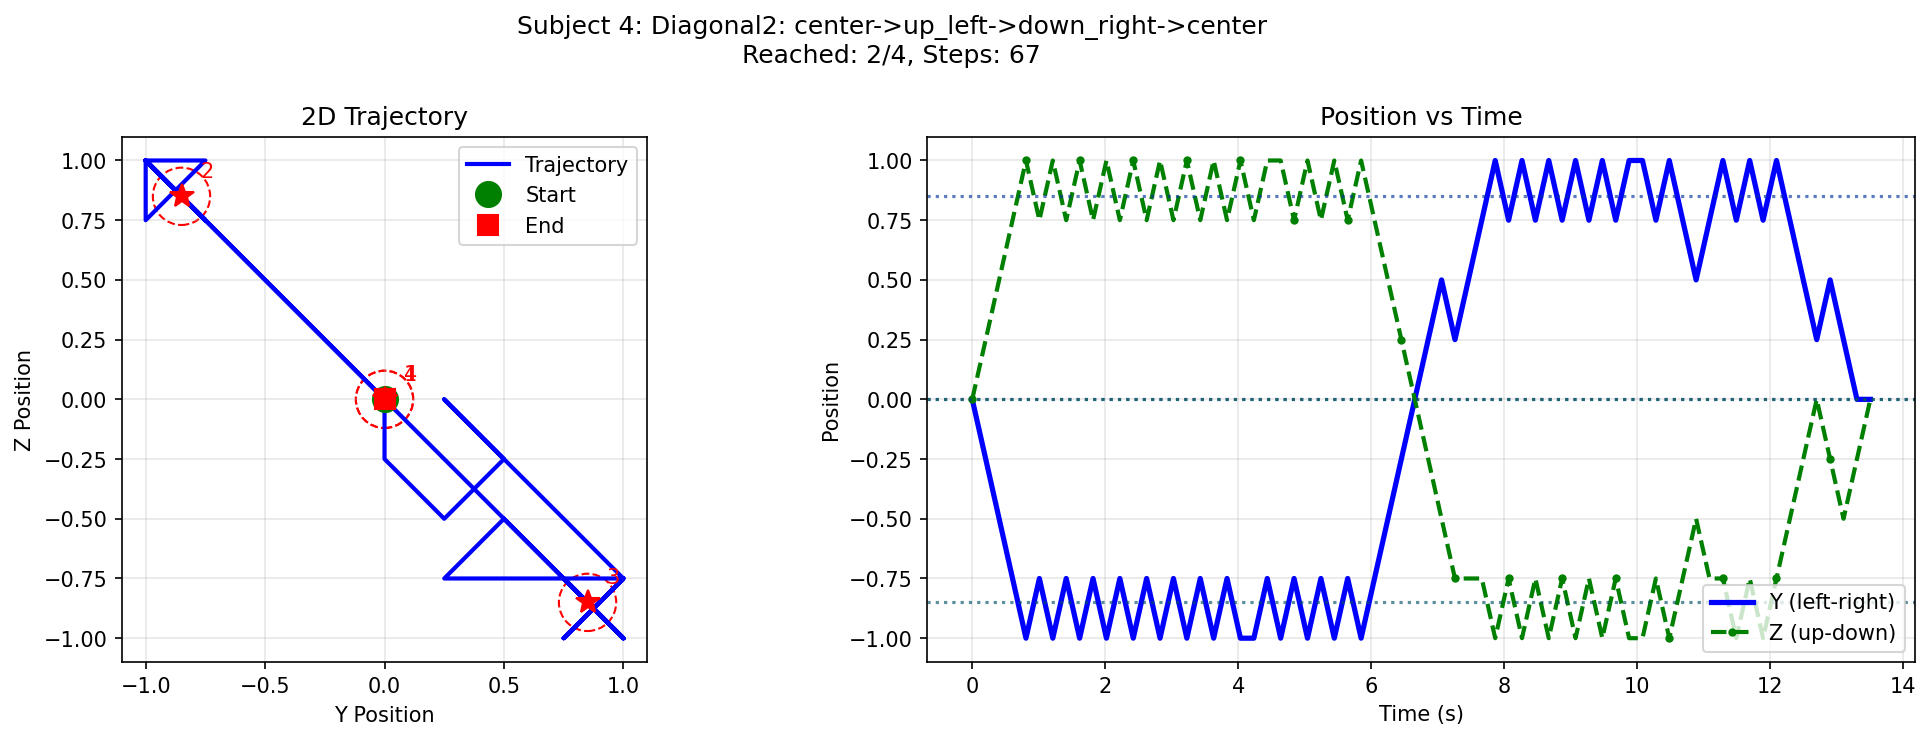
\includegraphics[width=\textwidth]{../outputs/eeg_physical_control/subject_4.png}
        \end{center}
        
        \column{0.33\textwidth}
        \textbf{Subject 5 (Square CW):}
        \begin{center}
            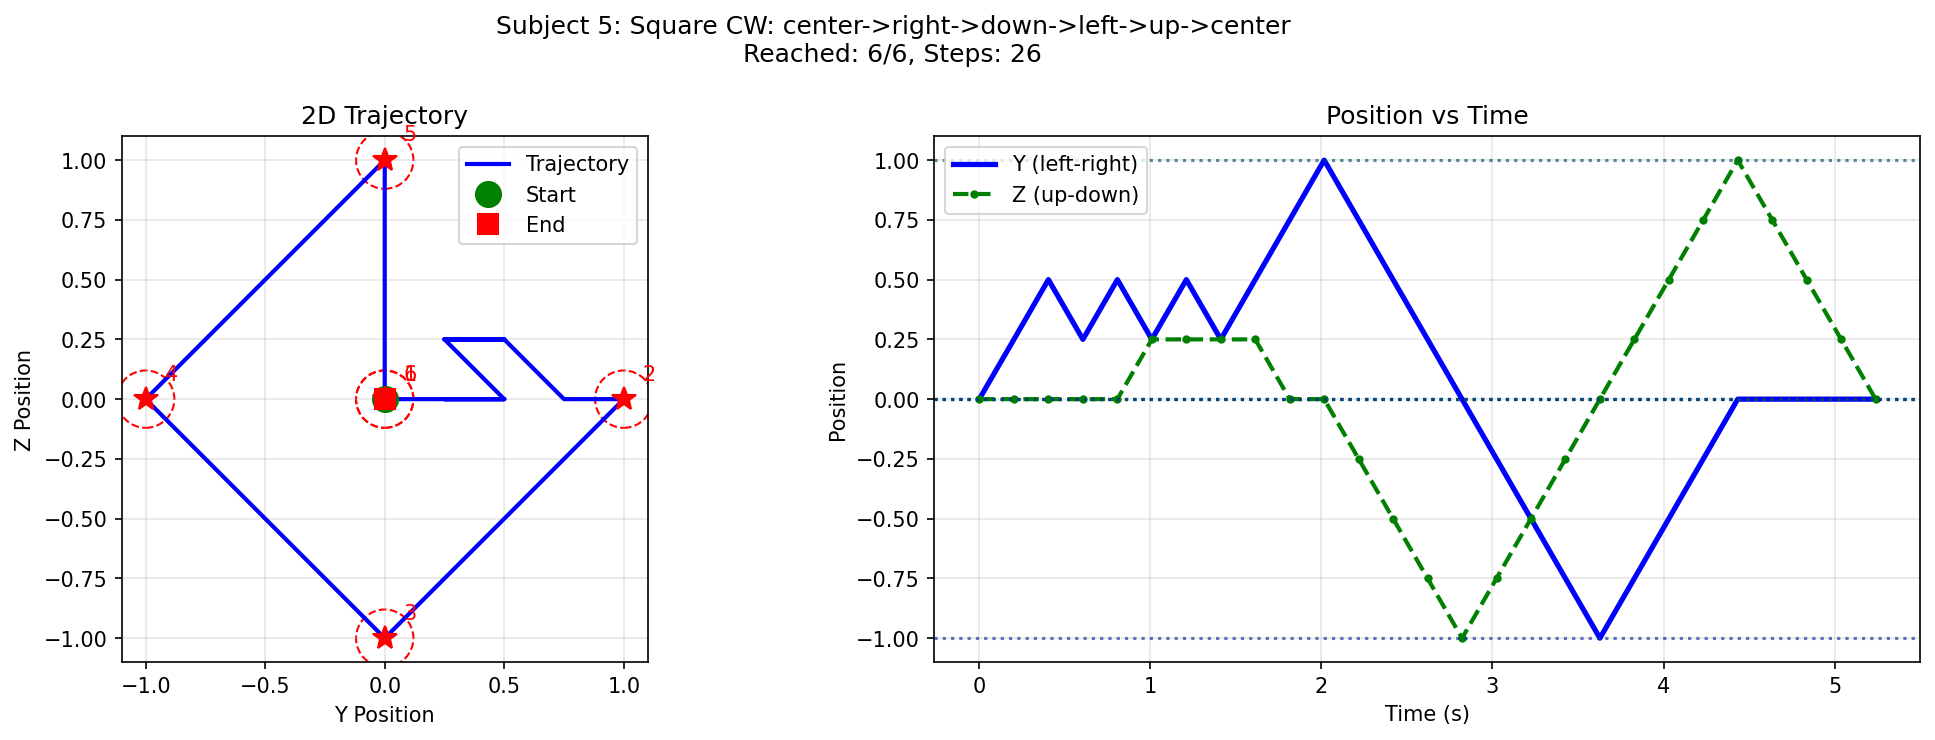
\includegraphics[width=\textwidth]{../outputs/eeg_physical_control/subject_5.png}
        \end{center}
        
        \column{0.33\textwidth}
        \textbf{Subject 6 (Square CCW):}
        \begin{center}
            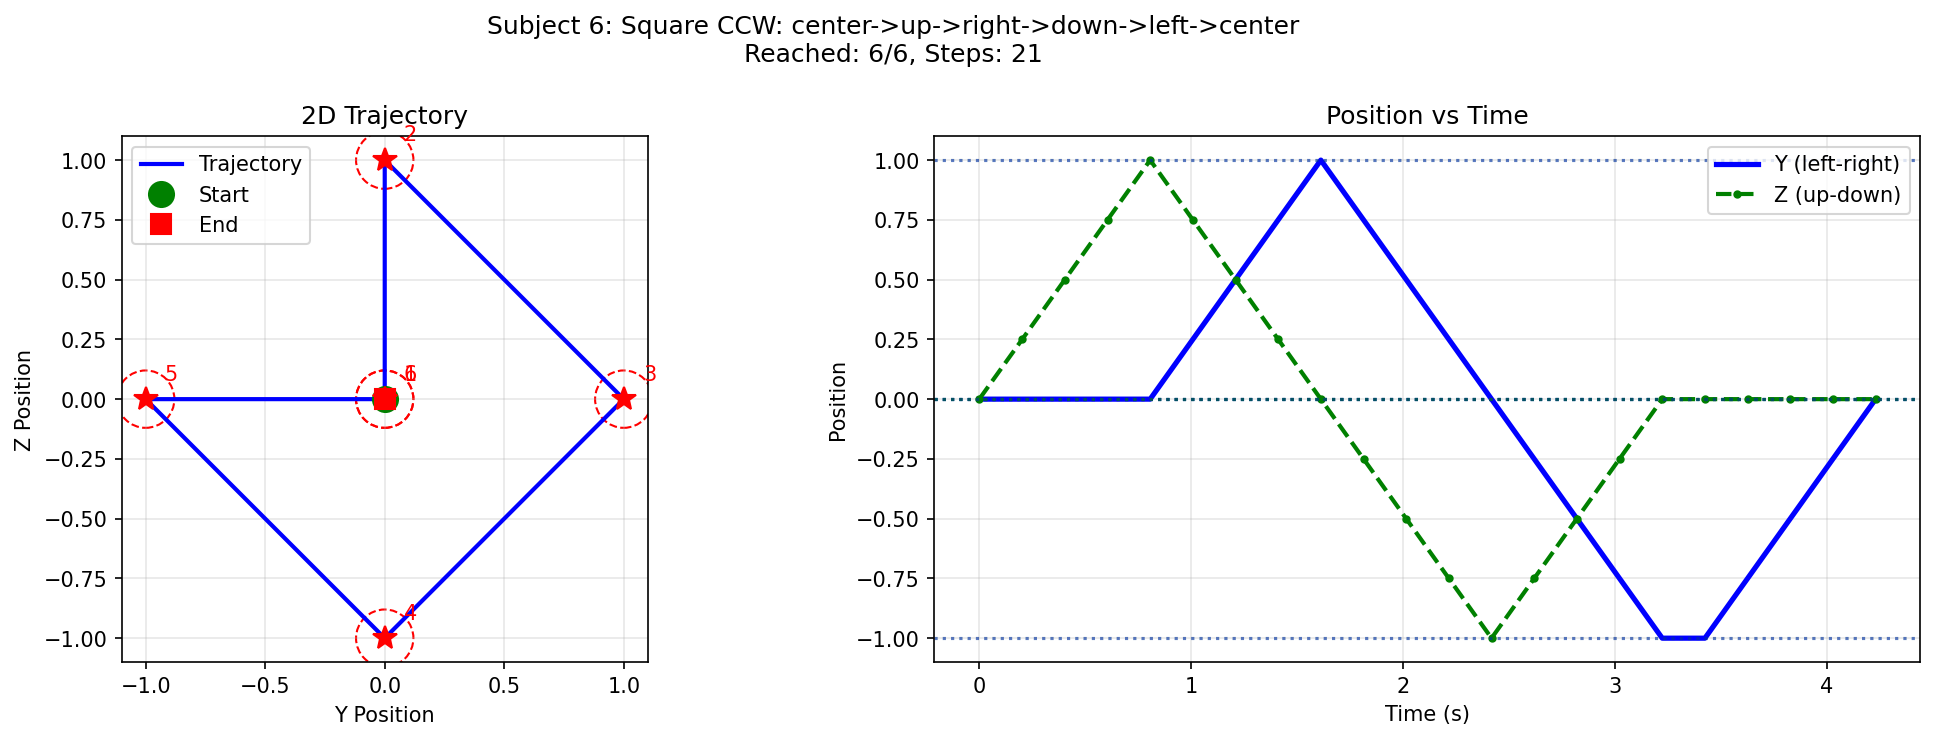
\includegraphics[width=\textwidth]{../outputs/eeg_physical_control/subject_6.png}
        \end{center}
    \end{columns}
    
    \vspace{2mm}
    \textbf{Note:} Complex patterns (square) require more steps due to multiple targets
\end{frame}

% ========== Slide 10: Comparison - EEG vs Physical Test ==========
\begin{frame}{Comparison: EEG Control vs Physical Test Baseline}
    \begin{center}
        
\includegraphics[width=0.9\textwidth]{../outputs/eeg_physical_control/comparison.png}
    \end{center}
    
    \textbf{Analysis:} Solid lines = EEG-based control, Dashed lines = Physical test baseline
\end{frame}

% ========== Slide 11: Error Analysis ==========
\begin{frame}{Error Analysis: EEG Control --- Endpoint Error}
    \begin{columns}[T]
        \column{0.48\textwidth}
        \begin{center}
            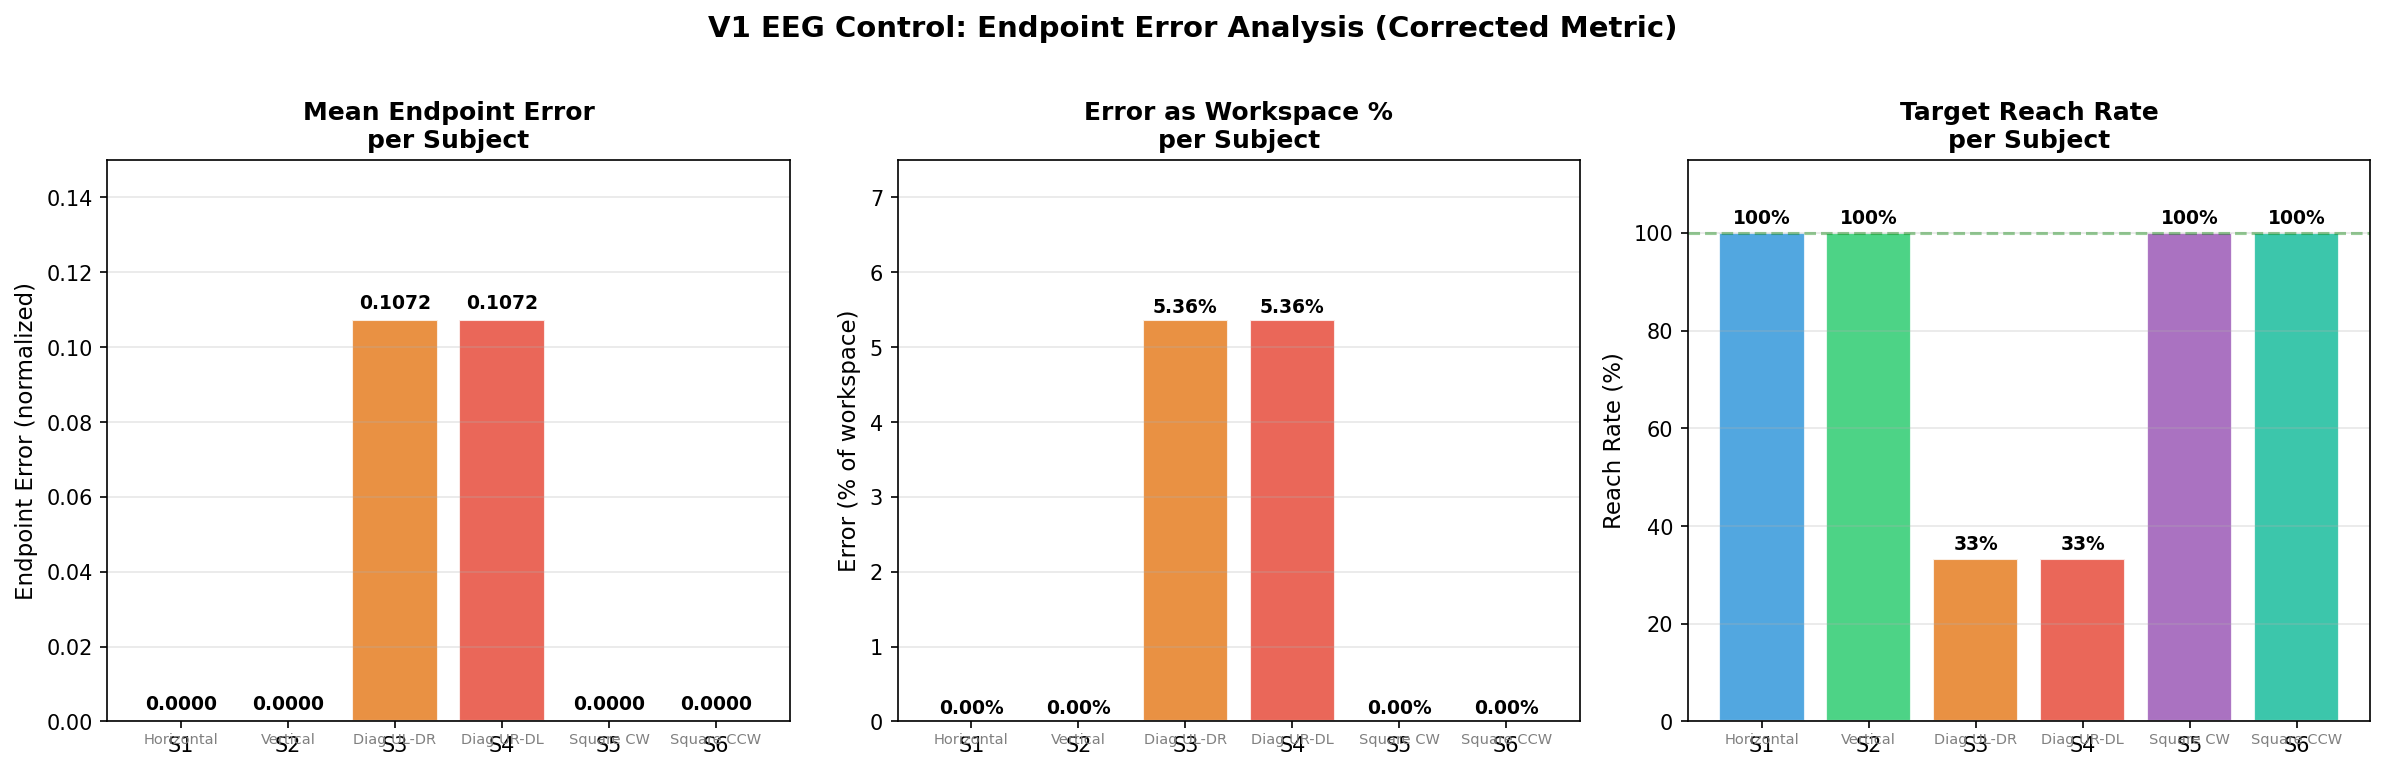
\includegraphics[width=\textwidth,height=0.55\textheight,keepaspectratio]{../outputs/eeg_physical_control/error_analysis_endpoint.png}
        \end{center}
        
        \column{0.52\textwidth}
        \textbf{Metric:} Endpoint Error $d = \sqrt{(\Delta y)^2 + (\Delta z)^2}$
        
        \vspace{1mm}
        \begin{table}
            \centering
            \scriptsize
            \begin{tabular}{lcc}
                \toprule
                Subject & Error & Workspace\% \\
                \midrule
                S1--S2 (Horiz/Vert) & 0.000 & 0.00\% \\
                S3--S4 (Diagonal) & 0.107 & 5.36\% \\
                S5--S6 (Square) & 0.000 & 0.00\% \\
                \midrule
                \textbf{Mean} & \textbf{0.036} & \textbf{1.79\%} \\
                \bottomrule
            \end{tabular}
        \end{table}
    \end{columns}
    
    \vspace{1mm}
    \begin{block}{Error Unit}
    \footnotesize
    All errors: \textbf{endpoint error} (final distance to target) in normalized coordinates $[-1, 1]$. \\
    Workspace\% $= \frac{\text{error}}{2.0} \times 100\%$. V1 step: $0.12$ norm $= 0.35$ rad ($20.1^\circ$). Reach threshold: $< 0.12$ (6\%).
    \end{block}
\end{frame}

% ========== Slide 12: Technical Challenges ==========
\begin{frame}{Challenges \& Solutions}
    \begin{columns}[T]
        \column{0.5\textwidth}
        \begin{alertblock}{Challenges Encountered}
            \begin{itemize}
                \item Joints not arriving simultaneously
                \item Wrist Flex slower due to load
                \item GOAL\_TIME conflicts (500ms vs 4000ms)
                \item Torque disabled causing drift
            \end{itemize}
        \end{alertblock}
        
        \column{0.5\textwidth}
        \begin{exampleblock}{Solutions Applied}
            \begin{itemize}
                \item Synchronized velocity calculation
                \item Velocity boost (1.3x-1.5x) for loaded joints
                \item Unified move\_time\_ms = 2000ms
                \item Keep torque enabled during close()
            \end{itemize}
        \end{exampleblock}
    \end{columns}
    
    \vspace{3mm}
    \textbf{Servo Velocity Compensation:}
    \begin{table}
        \centering
        \small
        \begin{tabular}{lcc}
            \toprule
            Joint & Base Velocity & Boosted Velocity \\
            \midrule
            Shoulder Lift & 300 & 390 (x1.3) \\
            Wrist Flex & 206 & 309 (x1.5) \\
            \bottomrule
        \end{tabular}
    \end{table}
\end{frame}

% ========== Slide 13: Results Summary ==========
\begin{frame}{Results Summary}
    \begin{columns}[T]
        \column{0.5\textwidth}
        \textbf{Physical Robot Testing:}
        \begin{table}
            \centering
            \small
            \begin{tabular}{lc}
                \toprule
                Metric & Value \\
                \midrule
                Patterns Tested & 6 \\
                Target Reach Rate & 100\% \\
                Motion Smoothness & High \\
                Joint Sync Error & $<$30 ticks \\
                \bottomrule
            \end{tabular}
        \end{table}
        
        \column{0.5\textwidth}
        \textbf{EEG-Based Control:}
        \begin{table}
            \centering
            \small
            \begin{tabular}{lc}
                \toprule
                Metric & Value \\
                \midrule
                Subjects Tested & 6 \\
                Noise Level & 10\% \\
                Mean Endpoint Error & 0.036 (1.79\%) \\
                Target Reach Rate & 81.8\% \\
                \bottomrule
            \end{tabular}
        \end{table}
    \end{columns}
    
    \vspace{5mm}
    \begin{block}{Key Achievement}
        Successfully demonstrated end-to-end BCI control pipeline from EEG simulation to physical robot movement with synchronized multi-joint control.
    \end{block}
\end{frame}

% ========== Slide 14: 下周计划 ==========
\begin{frame}{Next Week's Plan}
    \begin{block}{Planned Tasks}
        \begin{enumerate}
            \item Finalize report with all experimental results
            \item Generate performance comparison tables
            \item Create demonstration video of physical robot
            \item Complete project documentation
        \end{enumerate}
    \end{block}
    
    \vspace{5mm}
    
    \begin{columns}[T]
        \column{0.5\textwidth}
        \textbf{Expected Deliverables:}
        \begin{itemize}
            \item Final project report (draft)
            \item Demo video with all 6 patterns
            \item Performance metrics summary
        \end{itemize}
        
        \column{0.5\textwidth}
        \textbf{Project Status:}
        \begin{itemize}
            \item All core components complete
            \item Physical testing validated
            \item Focus shifting to documentation
        \end{itemize}
    \end{columns}
\end{frame}

% ========== Slide 15: 时间线 ==========
\begin{frame}{Project Timeline}
    \begin{center}
    \resizebox{0.9\textwidth}{!}{%
    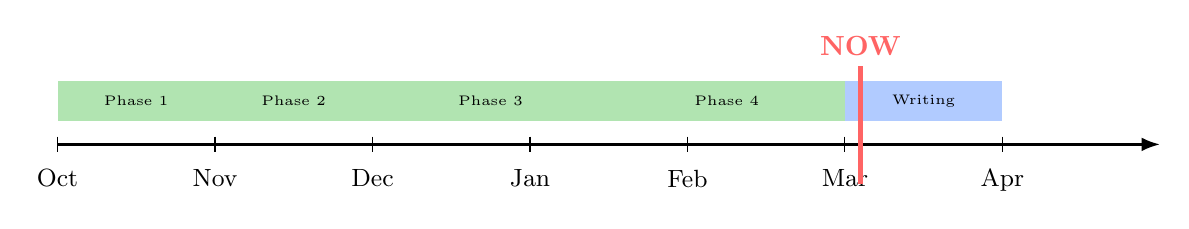
\begin{tikzpicture}
        % 时间轴
        \draw[thick, -Latex] (0,0) -- (14,0);
        
        % 月份标记
        \foreach \x/\month in {0/Oct, 2/Nov, 4/Dec, 6/Jan, 8/Feb, 10/Mar, 12/Apr} {
            \draw (\x, 0.1) -- (\x, -0.1);
            \node[below] at (\x, -0.2) {\small \month};
        }
        
        % 阶段块
        \fill[completed!50] (0, 0.3) rectangle (2, 0.8);
        \node at (1, 0.55) {\tiny Phase 1};
        
        \fill[completed!50] (2, 0.3) rectangle (4, 0.8);
        \node at (3, 0.55) {\tiny Phase 2};
        
        \fill[completed!50] (4, 0.3) rectangle (7, 0.8);
        \node at (5.5, 0.55) {\tiny Phase 3};
        
        \fill[completed!50] (7, 0.3) rectangle (10, 0.8);
        \node at (8.5, 0.55) {\tiny Phase 4};
        
        \fill[inprogress!50] (10, 0.3) rectangle (12, 0.8);
        \node at (11, 0.55) {\tiny Writing};
        
        % 当前位置
        \draw[highlight, ultra thick] (10.2, -0.5) -- (10.2, 1);
        \node[highlight, above] at (10.2, 1) {\textbf{NOW}};
        
    \end{tikzpicture}}
    \end{center}
    
    \vspace{3mm}
    \textbf{Current Status:} On track - All technical work complete, entering final documentation phase
\end{frame}

\end{document}
